\documentclass[11pt,a4paper]{report}

\usepackage[utf8]{inputenc}
\usepackage[french]{babel}
\usepackage{graphicx}

\author{Benjamin Pajusco et Paul ALNET}
\title{Systèmes électoraux: enjeux et  emplois au sein des démocraties}
\date{2020}

% Pour citer sans que cela n'aparaisse on utilise \nocite{bibid}
% On pourra éventuellement les changer automatiquement en \cite

% For the title background, via https://tex.stackexchange.com/questions/46280/how-to-create-a-background-image-on-title-page-with-latex
\usepackage{eso-pic}
\newcommand\BackgroundPic{%
	\put(0,-180){%
		\parbox[b][\paperheight]{\paperwidth}{%
			\vfill
			\centering
			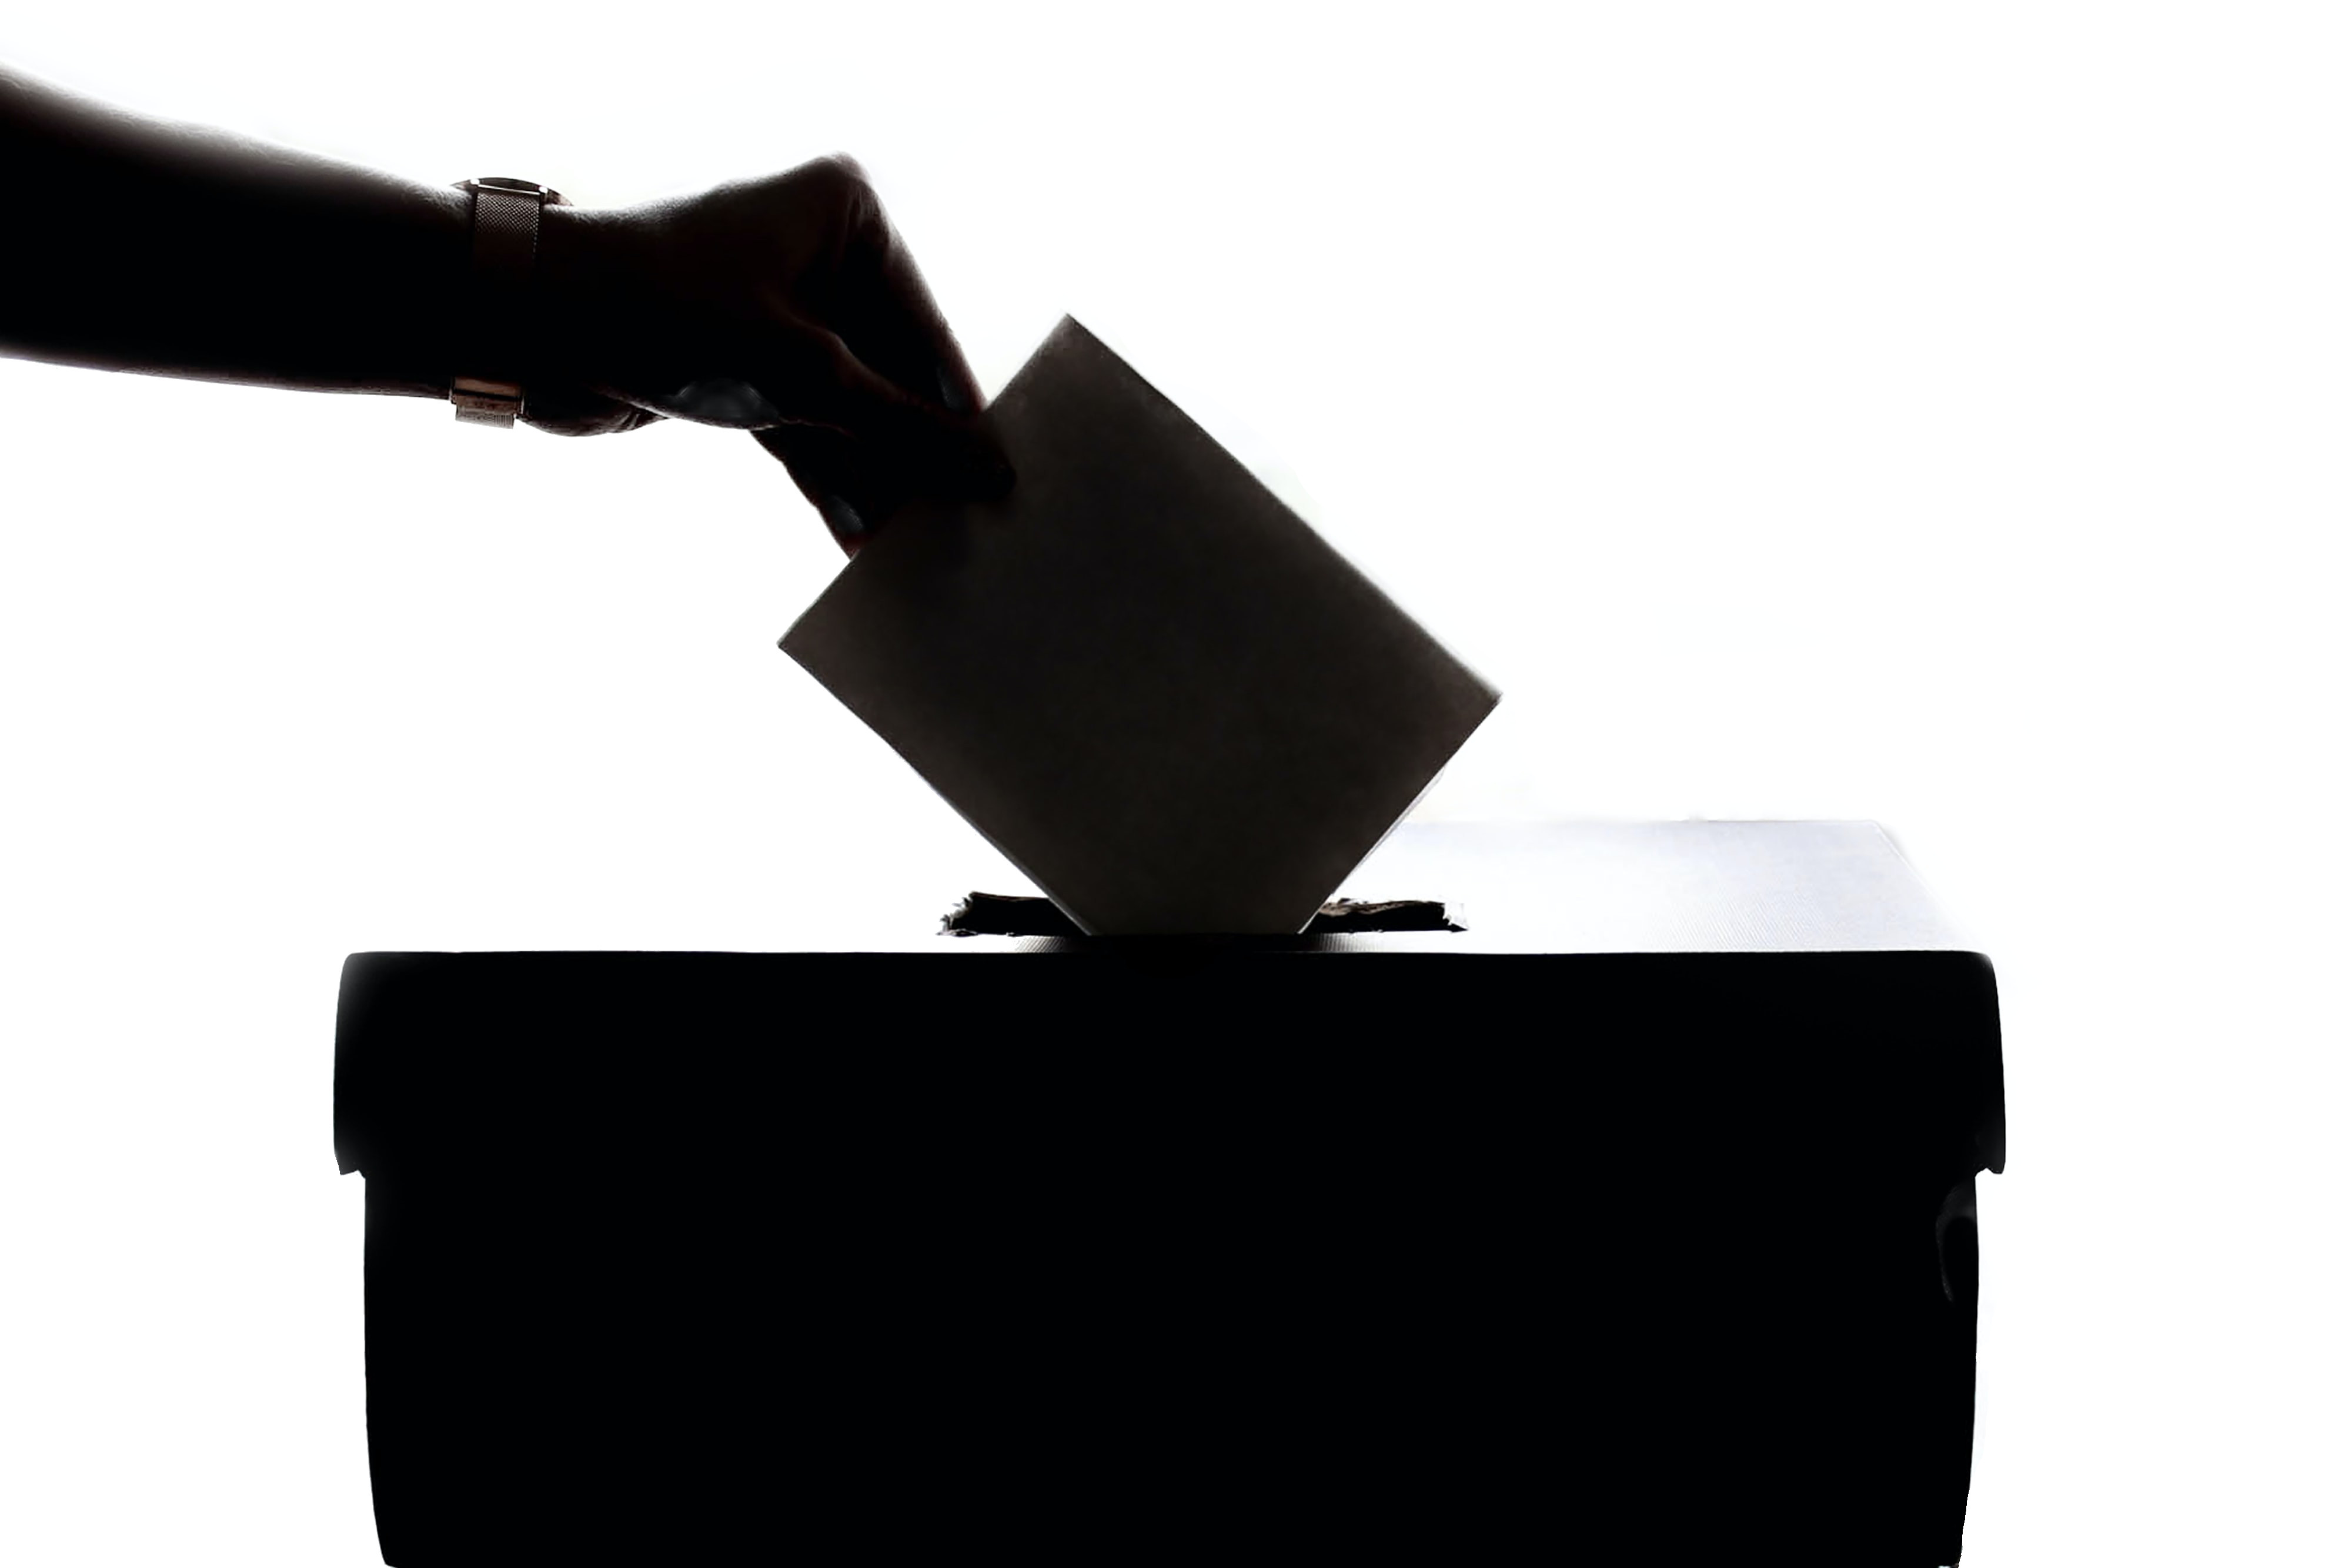
\includegraphics[width=\paperwidth,height=\paperheight,%
			keepaspectratio]{background.jpg}%
			\vfill
			
}}
	\put(100,36){\tiny{Photo par @element5digital sur Unsplash, légèrement altérée}}
}

\begin{document}
\AddToShipoutPicture*{\BackgroundPic}
\maketitle

\textbf{Quelles sont les différentes approches pour donner la voix au peuple, leurs évolutions et quelles sont les conséquences de leurs implémentations?}

\section*{Introduction}
 L'avenant des gouvernements, la transition progressive vers des états plus démocratiques, le pouvoir théoriquement donné au au peuple, nécessite l'apport d'une méthode pour permettre à chaque citoyen de faire entendre sa voix, son opinion. \nocite{wiki:demo}
 Chacun devant vaquer à ses occupations et ne pouvant pas investir temps et ressources dans la vie démocratique ainsi que la soif accrue du pouvoir détenue par certains font que l'on opte plutôt pour désigner des représentants du peuple, souvent par le biais d'élections; on appelle ceci la démocratie représentative. \nocite{wiki:seppv}
 Aristote déjà conçoit que celle-ci doit s'accompagner d'une séparation des pouvoirs. C'est à dire que les pouvoirs législatif, qui établit la loi et le budget de l'État, exécutif, qui applique la loi, et judiciaire, qui veille à la bonne application de la loi, sont partagés par différents groupes d'individus, au contraire d'une autocratie. \nocite{viepub:seppv}
 
 Ces personnes n'apparaissent pas magiquement, des procédés, variant selon les pays et régions, sont dictés dans les lois et sont suivis pour déterminer qui représentera, qui dirigera la nation.
 Nombreuses sont les organisations plaçant à la tête du pouvoir exécutif une hiérarchie menée par une personne élue, souvent président ou premier ministre, nommant les autres membres de la tête de l'administration. Il est généralement admis que cette personne dirigeante devrait être élue par le peuple, démocratiquement. 
 Ce défi logistique est confronté avec diverses approches selon les pays.
 


\tableofcontents

\chapter{L'évolution des systèmes de vote}
\nocite{wiki:histdemo}
Les modèles des démocraties modernes ne sont pas apparues instantanément mais découlent de plus de deux millénaires d'évolution.

\section{Démocratie Athénienne}
La capitale de la Grèce antique Athènes est reconnue comme l'une des premières origines de démocratie. En effet, au VI\up{e} siècle avant notre ère, la cité est, comme tant d'autres, confrontée à une crise politique. Pour y pallier, les législateurs renforcent le caractère démocratique du régime et rendent plus accessible la politique aux citoyens moins aisés en proposant notamment des compensations monétaires.

\subsection{Le corps électoral}
Si l'agglomération athénienne comptait 250 000 habitants\nocite{persee:popu}, seuls les citoyens peuvent voter. 
Or les femmes et esclaves n'étaient considérés que comme mineurs, seuls les fils de citoyen ayant suivi l'équivalent du service militaire moderne peuvent jouir du titre de citoyen.
 
Ces restrictions laissent un corps de 40 000 citoyens.



\chapter{Leurs emplois dans les démocraties contemporaines}

\newpage

\bibliography{bibliography} 
\bibliographystyle{ieeetr}

\end{document}
